\documentclass[a4paper,11pt,twoside,fleqn,openright]{memoir}
 
% Pakker
\usepackage[utf8]{inputenc} % Så må vi bruge æ, ø og å
%\usepackage[ansinew]{inputenc}
%\usepackage[danish]{babel} % Dansk opsætning
\usepackage[T1]{fontenc} % Hjælper med ordeling ved æ, ø og å. Sætter fontene til at være ps-fonte i stedet for bmp.
%\usepackage[scaled]{beramono} % Bedre monospace font
\usepackage{amsmath,amsfonts,amssymb} % God matematik
\usepackage{sistyle} % Enheder til fysik
\usepackage{array,booktabs} % Til gode tabeller
\usepackage{ragged2e} % For at kunnu lave tabeller med fast kolonnebredde, bruges sammen med 'array'
\usepackage{float} % Vi må nu bruge H som placering til floats
\usepackage{hhline} % Sum linie i tabel
\usepackage{multirow} % Fletning af rækker
\usepackage{multicol} % Fletning af kolonner
\usepackage{xcolor} % Vi kan bruge \color osv
\usepackage{colortbl} % Muligøre farver i tabeller
%\usepackage[danish=quotes]{csquotes} % Danske anførselstegn, brug enquote{}
\usepackage[english=british]{csquotes} 
\usepackage{graphicx} % Inkludere ekstern grafik
\usepackage[english,final]{varioref} % Vi kan anvende \vref
\usepackage{natbib} % Bedre litteratur henvisninger
\usepackage{pdfpages} % Inkludere en pdf side som en side  
\usepackage{acronym} % Smart akronymhåndtering
\usepackage{suffix} % Krævet af acronym
\usepackage{listings} % Til at inkludere kildekode direkte
\usepackage{lipsum} % Lorem ipsum dolar sit amet
\usepackage{caption} % Vi kan bruge \captionof
\usepackage{subfig} % Vi kan nu bruge \subfloat
\usepackage{calc} % Vi kan regne med tællere
\usepackage{changepage} % Vi kan ændre sidelayoutet lokalt
\usepackage{layout} % Vi kan se dimensionecne på vores layout med \layout
\usepackage[footnote,final,english,silent,nomargin]{fixme}
\usepackage[colorinlistoftodos]{todonotes}
\usepackage[pdftex,bookmarks=true,bookmarksnumbered=true]{hyperref} % Links i dokumentet
\usepackage{textcomp} % HVAD FANDEN GØR DENNE PAKKE?
\usepackage{threeparttable} % Så vi kan lave tablenotes (se latexbogen)
\usepackage{fixltx2e} % HVAD FANDEN GØR DENNE PAKKE?
\usepackage{minitoc} % Vi kan lave del inholdsfortegnelser forhåbentlig
\usepackage{enumitem} % Better lists
\usepackage{geometry}

% For sjov pakker
\usepackage{marvosym}
\usepackage{wasysym}
%\usepackage{fourier}

\captionsetup{font={small,sf},labelfont=bf}

\pagestyle{companion}

% Andre egensakber for komandoer
\newcommand\Cpp{C\raisebox{\height / 2}[\height][\depth]{\tiny ++}} % Pænere C++
\newcommand{\mimg}[4]{\marginpar{\small \centering{\includegraphics[width=#1]{#2}\captionof{figure}{\newline #3}\label{#4}}}} % Margin billede
\newcommand{\lmimg}[4]{\marginpar{\small\centering{% Latex margin billede
  \def\svgwidth{#1}
  \graphicspath{{illustrations/}}
  \input{illustrations/#2.pdf_tex}
  \captionof{figure}{\newline #3}
  \label{#4}}}
}
\newcommand{\mnote}[1]{\marginpar{\small \textsf{\textbf{Note}\\{#1}}}} % Margin note
\newcommand{\mcd}[1]{\marginpar{\textsf{\textbf{
\includegraphics[height=11pt]{frontmatter/media-optical}}\\\url{#1}}}} % CD-rom henvisning i margin
\newcommand{\cd}[1]{
\includegraphics[height=9pt]{frontmatter/media-optical}\url{#1}} % CD-rom henvisning i tekst
\newcommand{\limg}[5]{\begin{figure}[#1]
  \centering
  \def\svgwidth{#2}
  \graphicspath{{illustrations/}}
  \input{illustrations/#3.pdf_tex}
  \caption{#4}
	\label{#5}
\end{figure}}
\newcommand{\head}[1]{{\slshape{#1}}\vspace{5mm}} % Header
\newcommand{\tail}{\vspace{3mm}\fancybreak{$*\quad*\quad*$}\vspace{3mm}} % Røvhul
\newcommand{\enhed}[1]{\hfill\hbox{[#1]}\qquad} % At indsatte heb enheder i firkantparentes i "equation"
\newcommand{\dB}[0]{\hbox{dB}} % At skrive dB oprejst
%\addto\captionsdanish{
%\renewcommand\appendixname{Appendiks}
%\renewcommand\contentsname{Indholdsfortegnelse}

% Make vectors bold instead of a arrow
\let\oldhat\hat
\renewcommand{\vec}[1]{\mathbf{#1}}
\renewcommand{\hat}[1]{\oldhat{\mathbf{#1}}}

\makechapterstyle{box}{
  \renewcommand*{\printchaptername}{}
  \renewcommand*{\chapnumfont}{\normalfont\sffamily\huge\bfseries}
  \renewcommand*{\printchapternum}{
    \flushleft
    \begin{tikzpicture}[line width=4pt]
      \draw (0,1) -- (0,0) -- (1,0);
      \draw (2,1) -- (2,2) -- (1,2);
      \draw[color=gray] (1cm,1cm) node { \chapnumfont\thechapter };
    \end{tikzpicture}
  }
  \renewcommand*{\chaptitlefont}{\normalfont\sffamily\Huge\bfseries}
  \renewcommand*{\printchaptertitle}[1]{\flushleft\chaptitlefont##1}
  \setlength\beforechapskip{-100pt}
}

\newif\ifchapternonum
\makechapterstyle{nickoe}{
\renewcommand\printchapternonum{\chapternonumtrue}
  \renewcommand*{\printchaptername}{} % Removes the 'Chapter' text
  \renewcommand*{\chapnumfont}{\fontfamily{pbk}\fontseries{m} \fontshape{n}\fontsize{80}{35}\selectfont } % Does some magic
  \renewcommand*{\printchapternum}{}
  %\hfill 
  %\fontfamily{pbk}\fontseries{m} \fontshape{n}\fontsize{80}{35}\selectfont % Makes a gigantic number
  %\chapnumfont\thechapter} % Removes the 'Chapter's number
  \renewcommand*{\printchaptertitle}[1]{%
  \noindent%
  \ifchapternonum%
  \begin{tabularx}{\textwidth}{X}%
  {\parbox[b]{\linewidth}{\raggedright \hskip -0.6em \chaptitlefont ##1}%
    \vphantom{\raisebox{0pt}{\chapnumfont 1}}}
  \end{tabularx}%
  \else

  \begin{tabularx}{\textwidth}{Xl}
  {\parbox[b]{\linewidth}{\raggedright \hskip -0.6em \chaptitlefont ##1} }
  & \raisebox{0pt}{\raggedleft \chapnumfont \hskip -0.5cm \thechapter \hskip -0.5cm}%
  \end{tabularx}%
  \fi
  \hrule
  }

  %\flushleft\chaptitlefont##1} % Prints the chaptertitle
  %\renewcommand{\afterchaptertitle}{\par\nobreak\medskip\hrule\vskip\afterchapskip}
  \setlength\beforechapskip{-100pt} % Makes the chapter go up on the page

}

\newenvironment{ffk}[0]% formel forklaring
{\begin{list}{}%
         {\setlength{\leftmargin}{\mathindent}}%
         \item[]%
}
{\end{list}}

% Akronyms formatering
\renewcommand*{\acsfont}[1]{#1}
\renewcommand*{\acffont}[1]{#1}
\renewcommand*{\acfsfont}[1]{#1}

% Farve definitioner
\definecolor{shadecolor}{gray}{.95}

\lstloadlanguages{C,VHDL,Java}
% Kodeformatering [C]
\lstnewenvironment{ccode}[2][]{
  \def\lstlistingname{Source code}
  \lstset{
    language=C,
    escapeinside={(*@}{@*)},  % a line can set with: (*@\label{c:labelname}@*)
    keywordstyle=\bfseries,
    commentstyle=\color{blue}, 
    basicstyle=\ttfamily\selectfont\footnotesize,
    numbers=left,
    numberstyle=\tiny,
    tabsize=2,
    showstringspaces=false,
    backgroundcolor=\color{shadecolor},
    frame=lines,
    captionpos=b,
    caption={#1},
    label={#2}
  }
}{}

% Kodeformatering [VHDL]
\lstnewenvironment{VHDL}[2][]{
  \def\lstlistingname{Source code}
  \lstset{
    language=VHDL,
    keywordstyle=\bfseries,
    commentstyle=\color{blue}, 
    basicstyle=\ttfamily\selectfont\small,
    numbers=left,
    numberstyle=\tiny,
    tabsize=2,
    showstringspaces=false,
    backgroundcolor=\color{shadecolor},
    frame=lines,
    captionpos=b,
    caption={#1},
    label={#2}
  }
}{}

% Kodeformatering [Assembler]
\lstnewenvironment{asmcode}[2][]{
  \def\lstlistingname{Source code}
  \lstset{
    language=[x86masm]Assembler,
    keywordstyle=\bfseries,
    commentstyle=\color{blue}, 
    basicstyle=\ttfamily\selectfont\small,
    numbers=left,
    numberstyle=\tiny,
    tabsize=2,
    showstringspaces=false,
    breaklines=true,
    backgroundcolor=\color{shadecolor},
    frame=lines,
    captionpos=b,
    caption={#1},
    label={#2}
  }
}{}

% Kodeformatering [Java]
\lstnewenvironment{javacode}[2][]{
  \def\lstlistingname{Source code}
  \lstset{
    language=Java,
    keywordstyle=\bfseries,
    commentstyle=\color{blue}, 
    basicstyle=\ttfamily\selectfont\small,
    numbers=left,
    numberstyle=\tiny,
    tabsize=2,
    showstringspaces=false,
    breaklines=true,
    backgroundcolor=\color{shadecolor},
    frame=lines,
    captionpos=b,
    caption={#1},
    label={#2}
  }
}{}

% Kodeformatering [XML]
\lstnewenvironment{xmlcode}[2][]{
  \def\lstlistingname{Source code}
  \lstset{
    language=XML,
    keywordstyle=\bfseries,
    commentstyle=\color{blue},
    basicstyle=\ttfamily\selectfont\small,
    numbers=left,
    numberstyle=\tiny,
    showstringspaces=false,
    backgroundcolor=\color{shadecolor},
    frame=lines,
    morekeywords={msgid, repeat, mmsi, navstat, rot, sog, posaccu, lon, lat, cog, truehead, timestamp, manoeuvre, raim, commstate, utc_year, utc_month, utc_day, utc_hour, utc_min, utc_sec, txbcast, name, aisver, imo, call, cargo, a, b, c, d, fixdev, eta_mon, eta_day, eta,hour, eta_min, draught, dest, dte, spare},
    captionpos=b,
    breaklines=true,
    caption={#1},
    label={#2}
  }
}{}

% \part omdefinering, nu med beskrivende tekst
\def\descpart#1#2{
  \par\newpage\clearpage % Page break 
  \vspace*{5cm} % Vertical shift 
  \refstepcounter{part}% Next part
  %\addcontentsline{toc}{part}{\texorpdfstring{\rlap{\thepart}\hspace{1.2em}#1}{\thepart\ #1}} % Adds entry to TOC 
  \addcontentsline{toc}{part}{\texorpdfstring{\rlap{\thepart}\hspace{2em}#1}{\thepart\ #1}} % Adds entry to TOC 
  {\centering \textbf{\Huge Part \thepart}\par}
  \vspace{1cm} % Vertical shift
  \thispagestyle{chapter} % Gives the pagestile an the memoir chapterpagestyle
  {\centering \textbf{\Huge #1}\par}
  \begin{center}
  {\parbox{9cm}{
  \vspace{2cm} % Vertical shift
  \noindent \slshape{#2} % Some text
  }}
  \end{center}
  \vfill\pagebreak % Fill the end of page and page break
}

%------------
\def\appendixpart#1#2{
  \par\newpage\clearpage % Page break 
  \vspace*{5cm} % Vertical shift 
  \addcontentsline{toc}{part}{\texorpdfstring{\rlap{\thepart}\hspace{2em}#1}{\thepart\ #1}} % Adds entry to TOC 
  \thispagestyle{chapter} % Gives the pagestile an the memoir chapterpagestyle
  {\centering \textbf{\Huge #1}\par}
  \begin{center}
  {\parbox{9cm}{
  \vspace{2cm} % Vertical shift
  \noindent \slshape{#2} % Some text
  }}
  \end{center}
  \vfill\pagebreak % Fill the end of page and page break
}


%------------

% At bruge figurer der fylder mere end brødteksten
% Der defineres nogle ekstra længder
\newlength{\fullwidth}
\setlength{\fullwidth}{\textwidth}
\addtolength{\fullwidth}{\marginparsep}
\addtolength{\fullwidth}{\marginparwidth}
\newlength{\fullmargin}
\setlength{\fullmargin}{\marginparwidth}
\addtolength{\fullmargin}{\marginparsep}
% For at bruge det, skal man f.eks. gøre således:
%\begin{figure}[h]
%\begin{adjustwidth*}{-\fullmargin}{}
%\includegraphics[width=\fullwidth]{./sti}
%\end{adjustwidth*}
%\caption{Beskrivelse her}
%\laber{fig:label}
%\end{figure}

% \degC for grader C
% \arcdeg for gradtegn
\renewcommand{\epsilon}{\varepsilon}
\newcommand{\MATLAB}{M{\footnotesize ATLAB}}
\parindent 8pt

% Orddeling
% Ord der deles forkert kan skrives her, men bindestreg ved stavelser og mellemrum mellem ordene
\hyphenation{ar-bejds-in-ten-si-ve an-grebs-vink-ler ind-gangs-im-pe-dans ro-ta-ti-ons-en-ko-der deres clock-fre-kvens sys-tem-et na-vi-gate} 


\hypersetup{
  pdftitle={AAUB\AA D},
  pdfsubject={6th semester of Electronics and IT, Aalborg University},
  pdfauthor={Brian Bach Nielsen, Nick \O stergaard, Simon Als Nielsen, Rasmus Lundgaard Christensen and Christoffer Stagsted Andreassen},
  pdfcreator=LaTeX,
  linkcolor=black,
  citecolor=black,
  filecolor=black,
  urlcolor=black
}

\begin{document}

% Frontpage
\author{Nick Østergaard and Jeppe Dam}
\title{\textbf{\emph{Formation Control for Unmanned Surface Vehicles for Surveying Purposes}}}
\date{\today}
\maketitle
\thispagestyle{empty}
\begin{center}
	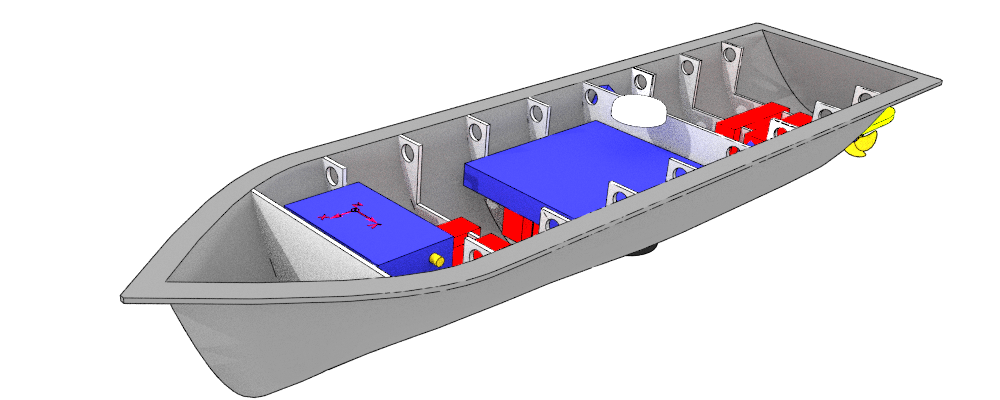
\includegraphics[width=13cm]{frontmatter/aauship}
\end{center}
\vfill
\begin{center}
	
\includegraphics[width=5cm]{frontmatter/AAU_LOGO_CMYK_UK}\\
	Department of Electronic Systems
\end{center}
\clearpage

\frontmatter
\chapterstyle{nickoe}

%\layout
%  \includepdf{illustrations/cover}
%\cleardoublepage
%\input{formalities/titelbladdk}
\cleardoublepage
\thispagestyle{empty}
\newgeometry{right=2cm}
\noindent
\begin{minipage}[l]{0.50\textwidth}
	\centering
	
\includegraphics[width=3.35cm]{frontmatter/AAU_LAT_CIRCLE_blue_rgb}
\end{minipage}
\begin{minipage}[r]{0.50\textwidth}

\noindent
	\begin{tabular}{l}
		{\textsf{\small \textbf{Institute of Electronic Systems}}}\\
		{\textsf{\small \textbf{Control Engineering}}} \\
		{\textsf{\small Fredrik Bajers vej 7}} \\
		{\textsf{\small 9220 Aalborg \O st}} \\
		{\textsf{\small Phone 99 40 86 00}} \\
		{\textsf{\small http://es.aau.dk}}
	\end{tabular}
\end{minipage}


%\fbox{
\begin{minipage}[c]{0.45\textwidth}
	\begin{description}[leftmargin=\parindent+0.5em,labelindent=\parindent]
	\item [\textbf{Title:}] \tightlist
	\item Formation Control of Autonomous Surface Vehicles for Surveying Purposes
	\end{description}

	\begin{description}
	\item [\textbf{Theme:}] \tightlist
	\item Master’s thesis
	\end{description}

	\begin{description}
	\item[Projectperiod:] \tightlist
	\item 2014
	\end{description}
	%  \hspace{4cm}
	\begin{description}
	\item[Projectgroup:] \tightlist
	\item 1034
	%  \hspace{4cm}
	\end{description}

	\begin{description}
	\item[Participants:] \tightlist
	\item Nick \O stergaard 
	\item Jeppe Dam
	\end{description} 

	\begin{description}
	\item[Supervisor:] \tightlist
	\item Jesper Abildgaard Larsen
	\end{description}

	\begin{description}
	\item[Number of printed copies:] 2
	\item[Number of pages:] \arabic{lastsheet} 
	\item[Appendices:] ??\todo{update} + website
		\footnote{Website with additional material, \url{http://kom.aau.dk/group/14gr1034/attached}}
	\item[Finished on:] \today
	\end{description}
\end{minipage}
\hfill
\begin{minipage}[r]{0.50\textwidth}
	{\textbf{Synopsis:}} \\
	\fbox{\parbox[c]{\textwidth-0.5em}{
	\bigskip
	{\vfill{\small \lipsum[1]

	\bigskip}}
    }}
\end{minipage}
%}
\vfill
\begin{center}
	
\includegraphics[width=1.35cm]{frontmatter/ca-logo.pdf}
\end{center}
\restoregeometry

%Rapporten skal afleveres til følgende:
%1 stk. til hovedvejlederen (afleveres til studiesekretæren)
%1 stk. til censor (afleveres til studiesekretæren)
%1 stk. til hver studerende i gruppen

\chapter{Preface}
\todo[inline]{This has to be written some time in the future, describe what this doc is.}

\subsubsection*{Thanks to}
\todo[inline]{Say thanks to someone, Aalborg Havn if they are helpfull? Karl D. has been glad to answer ROS related questions.}


\begin{center}
  \begin{minipage}[t]{0.47\textwidth}
    \centering \vspace{1.5cm} \hrule \vspace{1mm} Nick \O stergaard
  \end{minipage}
  \hfill
  \begin{minipage}[t]{0.47\textwidth}
    \centering \vspace{1.5cm} \hrule \vspace{1mm} Jeppe Dam
  \end{minipage}
\end{center}


\newpage
\section*{Reading guide}
The following report is divided into parts, related to different phases of the project. The parts are divided into chapters, the chapters describe different aspects of the project. The chapters are subdivided a number of times to further split up the content into specific topics. The report is ended with an appendix part, that contains all the material that is relevant to the project, but not necessarily interesting to the reader, such as measurement journals and transcripts of meetings.

\begin{description}
\item[Citations] in the report is done according to the Harvard method, the list of references can be found \vpageref{ch:litt}. The elements on the list of references are sorted by author.
\item[Acronyms] are written to their full extend, the first time they are used, with the acronym in parentheses, thereafter only the acronym is used. The list of acronyms can be found \vpageref{ch:acronyms}.
\item[Notation] of vectors are written in bold font with lower case letters ($\vec{v}$), matrices are written in bold font with upper case letters ($\vec{M}$). Single variables and constants are typeset in normal math ($x$).
\item[Attached] to the report is a CD, which contains copies of web references and other digital files (source code, scripts and raw measurement data) that could be of interest to the reader. In some places in the report there will be a reference to the CD; this will look like this: \cd{/path-to-file}.
\end{description}


%%%%%%% Maybe we should have an overview of the system here
\cleardoublepage
\tableofcontents
\chapter{Acronyms}
\label{ch:acronyms}
\begin{acronym}[TDMA]
%\begin{acronym}[HBCI]
	\acro{AAU}{Aalborg University}
  \acro{ASV}{Autonomous Surface Vessel}
	\acro{ADC}{Analog to Digital Converter}
  \acro{AHRS}{Attitude and Heading Reference System}
  \acro{BODY}{The body frame}
  \acro{CFD}{Computational Fluid Dynamics}
  \acro{DOF}{Degrees-Of-Freedom}
  \acro{DP}{Dynamic Positioning}
  \acro{ECEF}{Earth-Centered Earth-Fixed} 
  \acro{ECI}{Earth-Centered Inertial}
  \acro{EKF}{Extended Kalman Filter}
  \acro{FRF}{Formation Reference Frame}
  \acro{FRP}{Formation Reference Point}
	\acro{GNC}{Guidance, Navigation and Control}
  \acro{GNSS}{Global Navigation Satellite System}
  \acro{GPS}{Global Positioning System}
  \acro{GRS}{Ground Segment}
  \acro{HLI}{High Level Interface}
  \acro{IMU}{Inertial Measurement Unit}
	\acro{IP}{Internet Protocol}
	\acro{IPv4}{Internet Protocol version 4}
	\acro{IPv6}{Internet Protocol version 6}
  \acro{KF}{Kalman Filter}
  \acro{LKF}{Linear Kalman Filter}
  \acro{LOS}{Line-Of-Sight}
  \acro{LLI}{Low Level Interface}
	\acro{LSB}{Least Significant Bit}
  \acro{LTI}{Linear Time Invariant}
  \acro{MARG}{Magnetic, Angular Rate, and Gravity}
  \acro{MMSE}{Minimum Mean Square Error}
  \acro{MUV}{Multiple Unmanned Vehicle}
  \acro{MPC}{Model Predictive Control}
  \acro{NED}{North-East-Down}
  \acro{OSM}{OpenStreetMap}
  \acro{PWM}{Pulse Width Modulation}
  \acro{ROS}{Robot Operating System}
  \acro{RTK}{Real Time Kinematic}
  \acro{SOG}{Speed Over Ground}
  \acro{SSS}{Single Screw Ship}
  \acro{SSM}{State Space Model}
  \acro{TSS}{Twin Screw Ship}
  \acro{UGAS}{Uniformly Globally Asymptotically Stable}
  \acro{UGES}{Uniformly Globally Exponentially Stable}
  \acro{UGS}{Uniformly Globally Stable}
  \acro{UKF}{Unscented Kalman Filter}
  \acro{WGS84}{World Geodetic System 1984}
\end{acronym}



\mainmatter
\descpart{Preliminary analysis}{%
This is da stuff that is roolin'.}


\cleardoublepage
\descpart{Appendix}{%
The appendix includes chapters which are important for the project, but not necessarily interesting to the reader of the report.}
\appendix

%\input{appendix/filename}

%\input{appendix/fundapplication}


\backmatter
%\bibliography{formalities/litterature}
\label{ch:litt}

%\settocdepth{section}
%\listoftodos
\end{document}

